\title{Assignment 4: CS 736, Algorithms for Medical Image Processing}
\author{Alankar Kotwal -- 12D070010, Riddhish Bhalodia -- 120070003}

\documentclass[11pt]{article}

\usepackage{amsmath}
\usepackage{amssymb}
\usepackage{hyperref}
\usepackage{ulem}
\usepackage{graphicx}
\usepackage{float}
\usepackage[margin=0.5in]{geometry}

\begin{document}
\maketitle
\section*{Part (a)}
The selected value was $q=4$.

\section*{Part (b)}
The neighborhood mask, shown as an image, looks like the following: \\ \\
\centerline{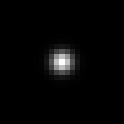
\includegraphics[scale=1]{weights}} \\ \\

\section*{Part (c)}
Initial memberships were put to $1/3$ for each class for each pixel. This was fixed because it is a natural condition to begin with.

\section*{Part (d)}
Initial class means were fixed to 0, 0.5 and 1. The reason behind this was to make sure that the initial means were well-separated and covered the entire range of intensities.

\section*{Part (f)}
Corrupted image: \\ \\
\centerline{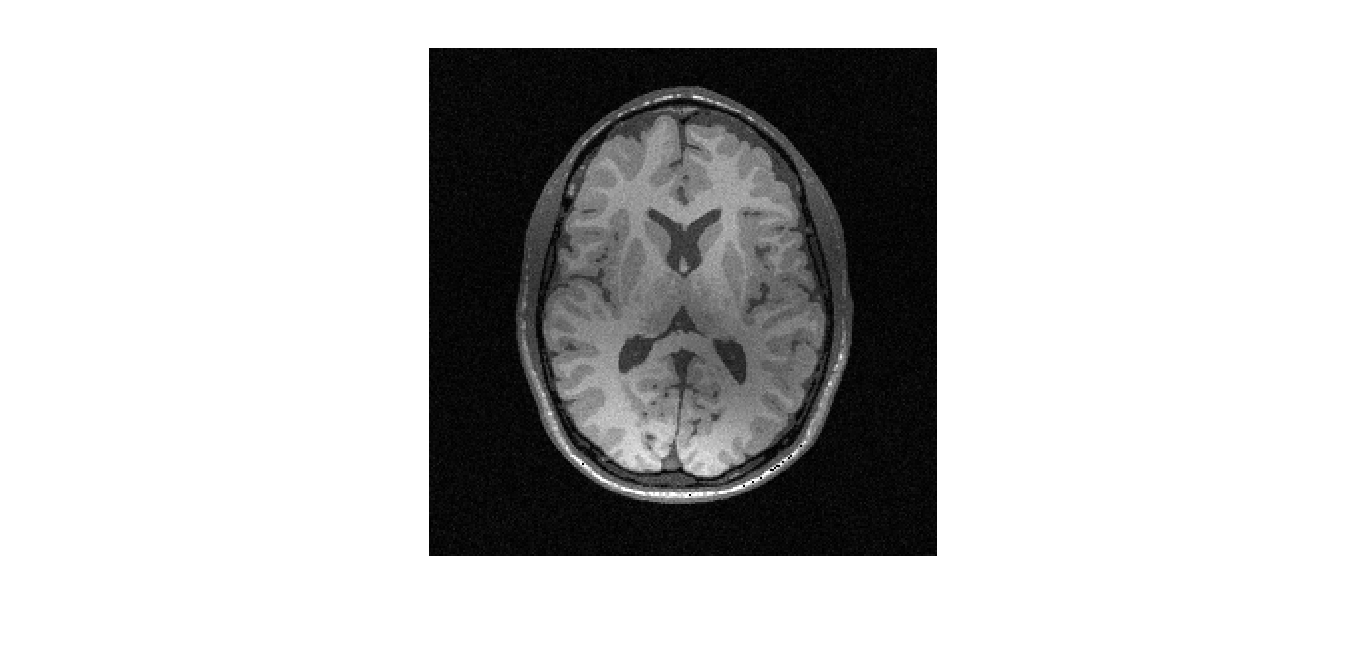
\includegraphics[scale=0.5]{corruptImage}} \\ \\
Optimal class-membership image: \\ \\
\centerline{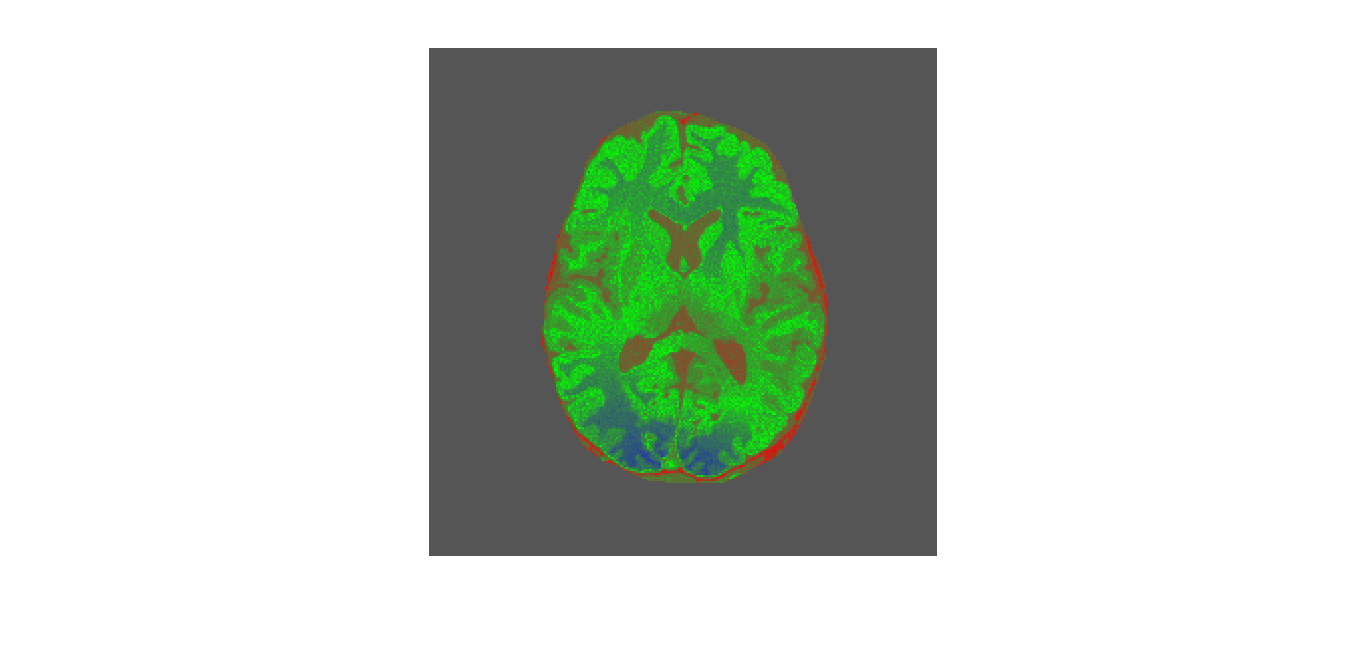
\includegraphics[scale=0.5]{mems}} \\ \\
Optimal bias-field estimate: \\ \\
\centerline{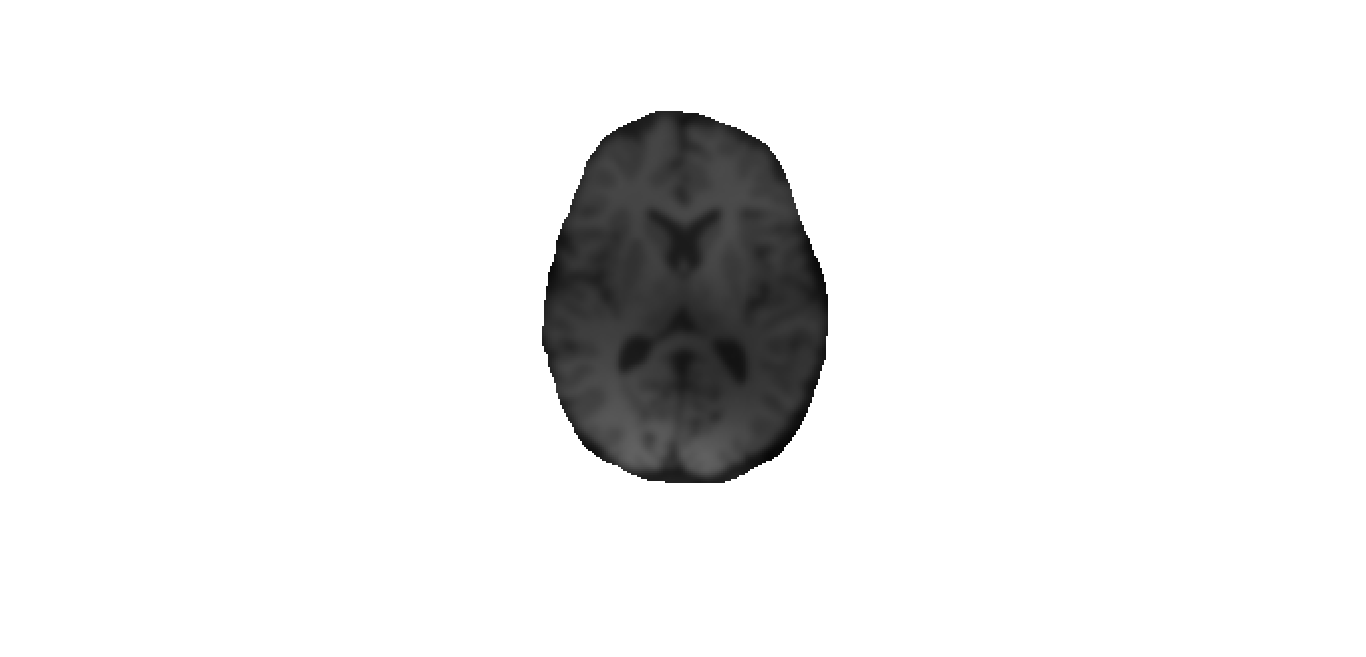
\includegraphics[scale=0.5]{bias}} \\ \\
Bias-removed image: \\ \\	
\centerline{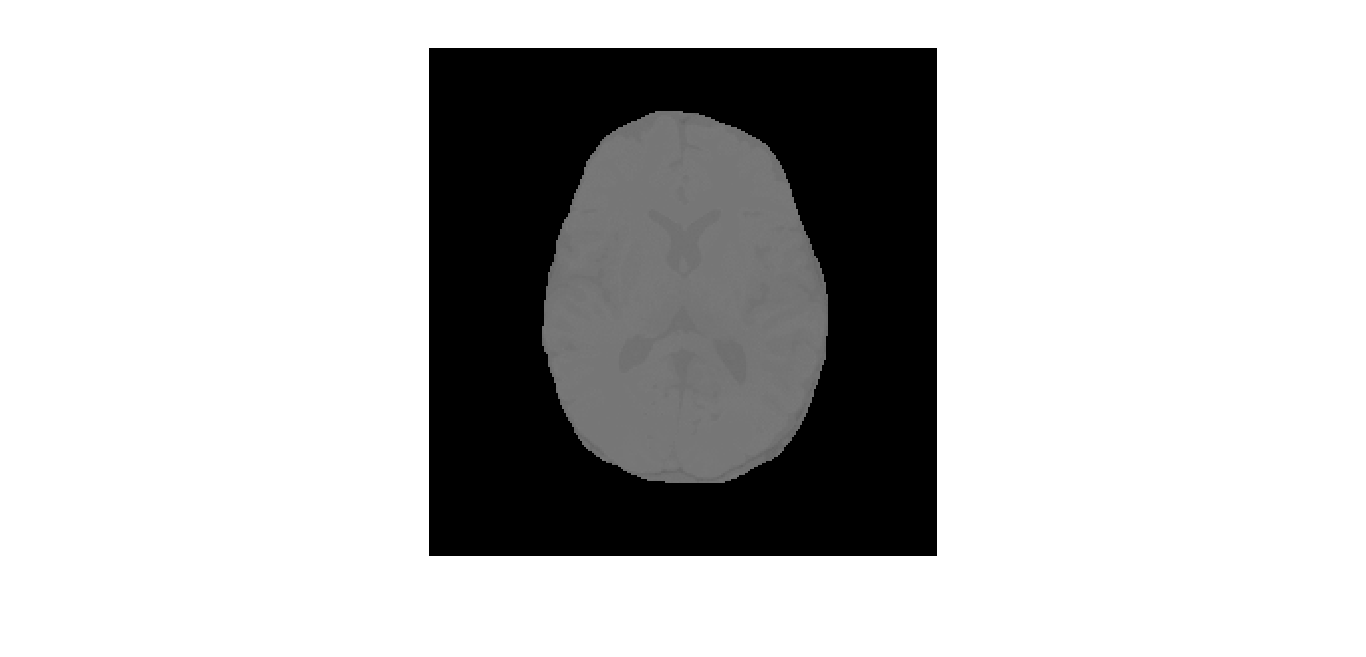
\includegraphics[scale=0.5]{biasRemoved}} \\ \\
Residual: \\ \\
\centerline{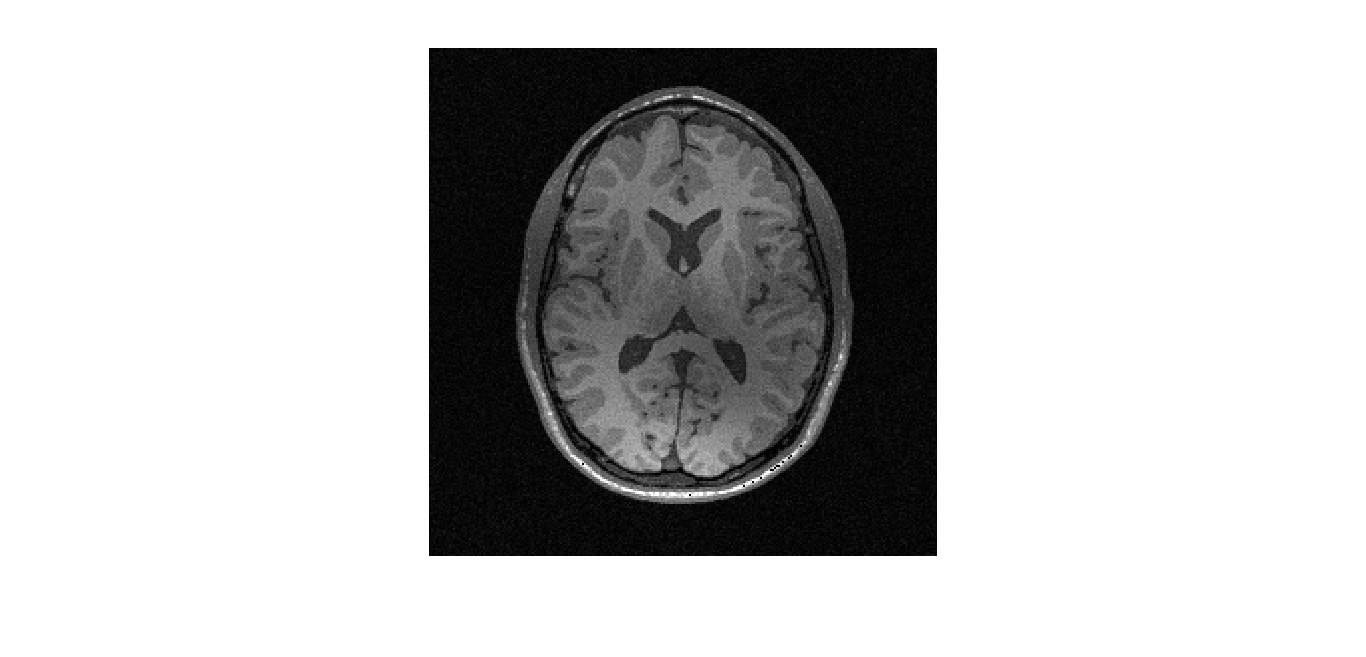
\includegraphics[scale=0.5]{residual}} \\ \\

\section*{Part (g)}
Class mean estimates: $[0.3908, 0.4742, 0.4887]$

\end{document}